\documentclass{article}
\usepackage[a4paper, top=2.5cm, bottom=2.5cm, left=2.5cm, right=2.5cm]{geometry}

\usepackage[utf8]{inputenc}

\usepackage{graphicx}
\usepackage{caption}
\usepackage{subcaption}
\usepackage{float}
\usepackage{amsmath}
\usepackage{multirow}


\usepackage{pgfplots}
\pgfplotsset{compat=1.18}

\usepackage{hyperref}

\usepackage{xcolor}
\usepackage{minted}

\definecolor{codebg}{RGB}{250, 250, 250}
\definecolor{codeframe}{RGB}{200, 200, 200}

\setminted{
    style=tango,
    fontsize=\footnotesize,
    bgcolor=codebg,
    linenos=false,
    breaklines=true,
    tabsize=4,
    frame=single,
    framesep=5pt,
    rulecolor=\color{codeframe},
}

\begin{document}

\title{
  \textbf{SDC Assignment 3 - Probability Bayesian}
}
\author{Ying Pei Lin}
\date{Spring 2026}

\maketitle

\section*{Exercise 2}

Suppose we live at a place where days are either sunny, cloudy, or rainy.
The weather transition function is a Markov chain with the following transition table:

\begin{center}
\begin{tabular}{|cc|ccc|}
\cline{3-5}
 \multicolumn{2}{c|}{} & \multicolumn{3}{c|}{tomorrow will be...} \\ % 使用 \multicolumn 控制上方空格的線條
 \multicolumn{2}{c|}{} & sunny & cloudy & rainy \\
\hline
\multirow{3}{*}{today it's...}
& sunny  & .8 & .2 & 0 \\
& cloudy & .4 & .4 & .2 \\
& rainy  & .2 & .6 & .2 \\
\hline
\end{tabular}
\end{center}

\begin{enumerate}
    \item[(a)] Suppose Day 1 is a sunny day. What is the probability of the following sequence of days:
    Day 2 = \textit{cloudy}, Day 3 = \textit{cloudy}, Day 4 = \textit{rainy}?

    \textbf{Answer:}

    $
    Seq = \{\text{Day 1 = \textit{sunny}}, \text{Day 2 = \textit{cloudy}}, \text{Day 3 = \textit{cloudy}}, \text{Day 4 = \textit{rainy}}\}
    $

    $
    P(\text{Day 2 = \textit{cloudy}} \mid \text{Day 1 = \textit{sunny}}) = 0.2
    $

    $
    P(\text{Day 3 = \textit{cloudy}} \mid \text{Day 2 = \textit{cloudy}}) = 0.4
    $

    $
    P(\text{Day 4 = \textit{rainy}} \mid \text{Day 3 = \textit{cloudy}}) = 0.2
    $

    $
    \begin{aligned}
    P(\text{Seq})
    &= P(\text{Day 2 = \textit{cloudy}} \mid \text{Day 1 = \textit{sunny}}) \cdot P(\text{Day 3 = \textit{cloudy}} \mid \text{Day 2 = \textit{cloudy}}) \\
    &\quad \cdot P(\text{Day 4 = \textit{rainy}} \mid \text{Day 3 = \textit{cloudy}}) \\
    &= 0.2 \cdot 0.4 \cdot 0.2 \\
    &= 0.016
    \end{aligned}
    $

    The probability of the sequence is 0.016.

    \item[(b)] Write a simulator that can randomly generate sequences of ``weathers'' from this state transition function.

    \textbf{Answer:}

    \begin{listing}[H]
        \caption{Weather Markov Chain Simulation}
        \label{lst:weather_sim}
        \begin{minted}{python}
        import random
        from enum import StrEnum, auto

        class Weather(StrEnum):
            SUNNY = auto()
            CLOUDY = auto()
            RAINY = auto()

        transitions = {
            Weather.SUNNY: {Weather.SUNNY: 0.8, Weather.CLOUDY: 0.2, Weather.RAINY: 0.0},
            Weather.CLOUDY: {Weather.SUNNY: 0.4, Weather.CLOUDY: 0.4, Weather.RAINY: 0.2},
            Weather.RAINY: {Weather.SUNNY: 0.2, Weather.CLOUDY: 0.6, Weather.RAINY: 0.2},
        }

        def weather_sim(init_weather, days):
            current_weather = init_weather
            sequence = [current_weather]

            for _ in range(days - 1):
                next_weather = random.choices(
                    population=list(transitions[current_weather].keys()),
                    weights=list(transitions[current_weather].values()),
                    k=1
                )[0]
                sequence.append(next_weather)
                current_weather = next_weather

            return sequence

        result = weather_sim(Weather.SUNNY, 10)
        print("Generated weather sequence:")
        for i, weather in enumerate(result, start=1):
            print(f"Day {i}: {weather.value}")
        \end{minted}
    \end{listing}

    \begin{figure}[H]
    \centering
    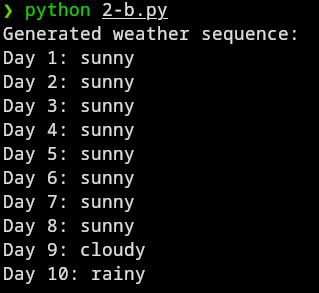
\includegraphics[width=0.4\textwidth]{2-b.png}
    \caption{Screenshot of the weather simulator generating a sequence of weathers.}
    \label{fig:weather_sim}
    \end{figure}

    \item[(c)] Use your simulator to determine the stationary distribution of this Markov chain. The stationary distribution measures the probability that a random day will be sunny, cloudy, or rainy.

        \textbf{Answer:}

        \begin{listing}[H]
        \caption{Weather Markov Chain Stationary Distribution}
        \label{lst:weather_sim_stationary}
        \begin{minted}{python}
            total_days = 1_000_000
            simulated_data = weather_sim(Weather.SUNNY, total_days)

            counts = Counter(simulated_data)
            stationary_dist = {state: count / total_days for state, count in counts.items()}

            print(f"Stationary Distribution after {total_days} days:")
            for state in Weather:
                print(f"{state.value.capitalize()}: {stationary_dist[state]:.4f}")
        \end{minted}
    \end{listing}

    \begin{figure}[H]
    \centering
    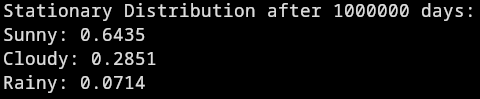
\includegraphics[width=0.4\textwidth]{2-c.png}
    \caption{Screenshot of the weather simulator calculating the stationary distribution.}
    \label{fig:weather_sim_stationary}
    \end{figure}

    \item[(d)] Can you devise a closed-form solution to calculating the stationary distribution based on the state transition matrix above?

    \textbf{Answer:}

    Let the stationary distribution be $\pi = [\pi_s, \pi_c, \pi_r]$. It must satisfy $\pi P = \pi$ and $\pi_s + \pi_c + \pi_r = 1$. Using the given transition matrix $P$, we establish the following system of equations:

    $$
    \begin{aligned}
    \pi P = \pi
    &\implies \begin{bmatrix} \pi_s & \pi_c & \pi_r \end{bmatrix}
    \begin{bmatrix}
    0.8 & 0.2 & 0 \\
    0.4 & 0.4 & 0.2 \\
    0.2 & 0.6 & 0.2
    \end{bmatrix}
    = \begin{bmatrix} \pi_s & \pi_c & \pi_r \end{bmatrix} \\
    &\implies
    \left\{
    \begin{aligned}
    0.8\pi_s + 0.4\pi_c + 0.2\pi_r &= \pi_s \\
    0.2\pi_s + 0.4\pi_c + 0.6\pi_r &= \pi_c \\
    0.2\pi_c + 0.2\pi_r &= \pi_r
    \end{aligned}
    \right.
    \end{aligned}
    $$

    From the third equation, solve for $\pi_c$:
    $$ 0.2\pi_c = 0.8\pi_r \implies \pi_c = 4\pi_r $$

    Substitute $\pi_c = 4\pi_r$ into the first equation to solve for $\pi_s$:
    $$ 0.8\pi_s + 0.4(4\pi_r) + 0.2\pi_r = \pi_s $$
    $$ 1.8\pi_r = 0.2\pi_s \implies \pi_s = 9\pi_r $$

    Apply the normalization constraint:
    $$ \pi_s + \pi_c + \pi_r = 1 $$
    $$ 9\pi_r + 4\pi_r + \pi_r = 1 $$
    $$ 14\pi_r = 1 \implies \pi_r = \frac{1}{14} $$

    Substitute $\pi_r$ back to find $\pi_s$ and $\pi_c$:
    $$ \pi_s = \frac{9}{14}, \quad \pi_c = \frac{4}{14} $$

    The closed-form stationary distribution is:
    $$ \pi = \left[ \frac{9}{14}, \frac{4}{14}, \frac{1}{14} \right] $$

    \item[(e)] What is the entropy of the stationary distribution?

    \textbf{Answer:}

    $$
    \begin{aligned}
    H(\pi) &= -\sum_{i} \pi_i \log_2(\pi_i) \\
    &= - \left( \frac{9}{14} \log_2 \frac{9}{14} + \frac{4}{14} \log_2 \frac{4}{14} + \frac{1}{14} \log_2 \frac{1}{14} \right) \\
    &\approx 1.198 \text{ bits}
    \end{aligned}
    $$

    \item[(f)] Using Bayes' rule, compute the probability table of yesterday’s weather given today’s weather. It is okay to provide the probabilities numerically, and it is also okay to rely on results from previous questions in this exercise.

    \textbf{Answer:}

    By Bayes' rule, the probability of yesterday's weather given today's weather is:
    $$
    P(W_{t-1} \mid W_t) = \frac{P(W_t \mid W_{t-1}) P(W_{t-1})}{P(W_t)}
    $$

    Assuming the Markov chain has reached its stationary distribution $\pi = \left[ \frac{9}{14}, \frac{4}{14}, \frac{1}{14} \right]$. The backward probability table is computed as follows:

    $$
    \begin{array}{c|ccc}
    W_t \setminus W_{t-1} & \text{Sunny} & \text{Cloudy} & \text{Rainy} \\
    \hline
    \text{Sunny} & 0.8 \cdot \frac{9/14}{9/14} = 0.8 & 0.4 \cdot \frac{4/14}{9/14} = \frac{8}{45} & 0.2 \cdot \frac{1/14}{9/14} = \frac{1}{45} \\[8pt]
    \text{Cloudy} & 0.2 \cdot \frac{9/14}{4/14} = 0.45 & 0.4 \cdot \frac{4/14}{4/14} = 0.4 & 0.6 \cdot \frac{1/14}{4/14} = 0.15 \\[8pt]
    \text{Rainy} & 0 \cdot \frac{9/14}{1/14} = 0 & 0.2 \cdot \frac{4/14}{1/14} = 0.8 & 0.2 \cdot \frac{1/14}{1/14} = 0.2
    \end{array}
    $$

    \item[(g)] Suppose we added seasons to our model. The state transition function above would only apply to the Summer, whereas different ones would apply to Winter, Spring, and Fall. Would this violate the Markov property of this process? Explain your answer.

    \textbf{Answer:}

    No, it would not violate the Markov property.

    The Markov property requires that the future state depends only on the current state, not on the sequence of past states.

    Adding seasons means the transition probabilities change depending on the time of year. As long as the prediction for tomorrow's weather relies only on today's weather and the current season, the Markov assumption holds.

\end{enumerate}

\section*{Exercise 3}

Suppose that we cannot observe the weather directly, but instead rely on a sensor.
The problem is that our sensor is noisy. Its measurements are governed by the following measurement model:

\begin{center}
\begin{tabular}{|cc|ccc|}
\cline{3-5}
 \multicolumn{2}{c|}{} & \multicolumn{3}{c|}{our sensor tells us...} \\
 \multicolumn{2}{c|}{} & sunny & cloudy & rainy \\
\hline
\multirow{3}{*}{the actual weather is...}
& sunny  & .6 & .4 & 0 \\
& cloudy & .3 & .7 & 0 \\
& rainy  & 0 & 0 & .1 \\
\hline
\end{tabular}
\end{center}

\begin{enumerate}
    \item[(a)] Suppose Day 1 is sunny (this is known for a fact), and in the subsequent four days our sensor observes \textit{cloudy}, \textit{cloudy}, \textit{rainy}, \textit{sunny}. What is the probability that Day 5 is indeed sunny as predicted by our sensor?

    \textbf{Answer:}

    Using the Bayes filter, let $Bel(X_t) = P(X_t \mid Z_{1:t})$:
    $$ \overline{Bel}(X_t) = P^T Bel(X_{t-1}) $$
    $$ Bel(X_t) = \eta \cdot P(Z_t \mid X_t) \odot \overline{Bel}(X_t) $$

    Given $Bel(X_1) = [1,\; 0,\; 0]^T$:

    \textbf{Day 2 ($Z_2 = \text{Cloudy}$):}
    $$ \overline{Bel}(X_2) = P^T Bel(X_1) = \begin{bmatrix} 0.8 & 0.4 & 0.2 \\ 0.2 & 0.4 & 0.6 \\ 0 & 0.2 & 0.2 \end{bmatrix} \begin{bmatrix} 1 \\ 0 \\ 0 \end{bmatrix} = \begin{bmatrix} 0.8 \\ 0.2 \\ 0 \end{bmatrix} $$
    $$ P(C \mid X_2) \odot \overline{Bel}(X_2) = \begin{bmatrix} 0.4 \\ 0.7 \\ 0 \end{bmatrix} \odot \begin{bmatrix} 0.8 \\ 0.2 \\ 0 \end{bmatrix} = \begin{bmatrix} 0.32 \\ 0.14 \\ 0 \end{bmatrix} $$
    $$ \eta_2 = \frac{1}{0.32 + 0.14 + 0} = \frac{1}{0.46} = \frac{50}{23} $$
    $$ Bel(X_2) = \frac{50}{23} \begin{bmatrix} 0.32 \\ 0.14 \\ 0 \end{bmatrix} = \begin{bmatrix} 16/23 \\ 7/23 \\ 0 \end{bmatrix} $$

    \textbf{Day 3 ($Z_3 = \text{Cloudy}$):}
    $$ \overline{Bel}(X_3) = P^T Bel(X_2) = \begin{bmatrix} 0.8 & 0.4 & 0.2 \\ 0.2 & 0.4 & 0.6 \\ 0 & 0.2 & 0.2 \end{bmatrix} \begin{bmatrix} 16/23 \\ 7/23 \\ 0 \end{bmatrix} = \frac{1}{23} \begin{bmatrix} 15.6 \\ 6.0 \\ 1.4 \end{bmatrix} $$
    $$ P(C \mid X_3) \odot \overline{Bel}(X_3) = \begin{bmatrix} 0.4 \\ 0.7 \\ 0 \end{bmatrix} \odot \frac{1}{23} \begin{bmatrix} 15.6 \\ 6.0 \\ 1.4 \end{bmatrix} = \frac{1}{23} \begin{bmatrix} 6.24 \\ 4.20 \\ 0 \end{bmatrix} $$
    $$ \eta_3 = \frac{23}{6.24 + 4.20 + 0} = \frac{23}{10.44} $$
    $$ Bel(X_3) = \frac{23}{10.44} \cdot \frac{1}{23} \begin{bmatrix} 6.24 \\ 4.20 \\ 0 \end{bmatrix} = \begin{bmatrix} 52/87 \\ 35/87 \\ 0 \end{bmatrix} $$

    \textbf{Day 4 ($Z_4 = \text{Rainy}$):}
    $$ \overline{Bel}(X_4) = P^T Bel(X_3) = \begin{bmatrix} 0.8 & 0.4 & 0.2 \\ 0.2 & 0.4 & 0.6 \\ 0 & 0.2 & 0.2 \end{bmatrix} \begin{bmatrix} 52/87 \\ 35/87 \\ 0 \end{bmatrix} = \frac{1}{87} \begin{bmatrix} 55.6 \\ 24.4 \\ 7.0 \end{bmatrix} $$
    $$ P(R \mid X_4) \odot \overline{Bel}(X_4) = \begin{bmatrix} 0 \\ 0 \\ 0.1 \end{bmatrix} \odot \frac{1}{87} \begin{bmatrix} 55.6 \\ 24.4 \\ 7.0 \end{bmatrix} = \frac{1}{87} \begin{bmatrix} 0 \\ 0 \\ 0.7 \end{bmatrix} $$
    $$ \eta_4 = \frac{87}{0.7} $$
    $$ Bel(X_4) = \frac{87}{0.7} \cdot \frac{1}{87} \begin{bmatrix} 0 \\ 0 \\ 0.7 \end{bmatrix} = \begin{bmatrix} 0 \\ 0 \\ 1 \end{bmatrix} $$

    \textbf{Day 5 ($Z_5 = \text{Sunny}$):}
    $$ \overline{Bel}(X_5) = P^T Bel(X_4) = \begin{bmatrix} 0.8 & 0.4 & 0.2 \\ 0.2 & 0.4 & 0.6 \\ 0 & 0.2 & 0.2 \end{bmatrix} \begin{bmatrix} 0 \\ 0 \\ 1 \end{bmatrix} = \begin{bmatrix} 0.2 \\ 0.6 \\ 0.2 \end{bmatrix} $$
    $$ P(S \mid X_5) \odot \overline{Bel}(X_5) = \begin{bmatrix} 0.6 \\ 0.3 \\ 0 \end{bmatrix} \odot \begin{bmatrix} 0.2 \\ 0.6 \\ 0.2 \end{bmatrix} = \begin{bmatrix} 0.12 \\ 0.18 \\ 0 \end{bmatrix} $$
    $$ \eta_5 = \frac{1}{0.12 + 0.18 + 0} = \frac{1}{0.3} $$
    $$ Bel(X_5) = \frac{1}{0.3} \begin{bmatrix} 0.12 \\ 0.18 \\ 0 \end{bmatrix} = \begin{bmatrix} 0.4 \\ 0.6 \\ 0 \end{bmatrix} $$

    The probability that Day 5 is sunny is $\mathbf{0.4}$.

    \item[(b)] Once again, suppose Day 1 is known to be sunny. At Days 2 through 4, the sensor measures \textit{sunny}, \textit{sunny}, \textit{rainy}. For each of the Days 2 through 4, what is the most likely weather on that day? Answer the question in two ways: one in which only the data available to the day in question is used, and one in hindsight, where data from future days is also available.

    \textbf{Answer:}

    Based on the model, define the state transition matrices $P^T$ (forward) and $P$ (backward), along with the emission probability vectors $O_S = P(S \mid X)$ and $O_R = P(R \mid X)$ for states $[S, C, R]^T$:
    $$ P^T = \begin{bmatrix} 0.8 & 0.4 & 0.2 \\ 0.2 & 0.4 & 0.6 \\ 0 & 0.2 & 0.2 \end{bmatrix}, \quad P = \begin{bmatrix} 0.8 & 0.2 & 0 \\ 0.4 & 0.4 & 0.2 \\ 0.2 & 0.6 & 0.2 \end{bmatrix} $$
    $$ O_S = \begin{bmatrix} 0.6 \\ 0.3 \\ 0 \end{bmatrix}, \quad O_R = \begin{bmatrix} 0 \\ 0 \\ 0.1 \end{bmatrix} $$

    \textbf{Method 1: Filtering (Forward Pass)} \quad $\alpha_t = O_{Z_t} \odot (P^T \alpha_{t-1})$

    Given $\alpha_1 = [1,\ 0,\ 0]^T$:

    \textbf{Day 2 ($Z_2 = \text{Sunny}$):}
    $$ P^T \alpha_1 = \begin{bmatrix} 0.8 & 0.4 & 0.2 \\ 0.2 & 0.4 & 0.6 \\ 0 & 0.2 & 0.2 \end{bmatrix} \begin{bmatrix} 1 \\ 0 \\ 0 \end{bmatrix} = \begin{bmatrix} 0.8 \\ 0.2 \\ 0 \end{bmatrix} $$
    $$ \alpha_2 = O_S \odot (P^T \alpha_1) = \begin{bmatrix} 0.6 \\ 0.3 \\ 0 \end{bmatrix} \odot \begin{bmatrix} 0.8 \\ 0.2 \\ 0 \end{bmatrix} = \begin{bmatrix} 0.48 \\ 0.06 \\ 0 \end{bmatrix} $$
    $$ Bel(X_2) = \frac{1}{0.54} \begin{bmatrix} 0.48 \\ 0.06 \\ 0 \end{bmatrix} = \begin{bmatrix} 0.889 \\ 0.111 \\ 0 \end{bmatrix} \implies \textbf{MAP: Sunny} $$

    \textbf{Day 3 ($Z_3 = \text{Sunny}$):}
    $$ P^T \alpha_2 = \begin{bmatrix} 0.8 & 0.4 & 0.2 \\ 0.2 & 0.4 & 0.6 \\ 0 & 0.2 & 0.2 \end{bmatrix} \begin{bmatrix} 0.48 \\ 0.06 \\ 0 \end{bmatrix} = \begin{bmatrix} 0.408 \\ 0.12 \\ 0.012 \end{bmatrix} $$
    $$ \alpha_3 = O_S \odot (P^T \alpha_2) = \begin{bmatrix} 0.6 \\ 0.3 \\ 0 \end{bmatrix} \odot \begin{bmatrix} 0.408 \\ 0.12 \\ 0.012 \end{bmatrix} = \begin{bmatrix} 0.2448 \\ 0.036 \\ 0 \end{bmatrix} $$
    $$ Bel(X_3) = \frac{1}{0.2808} \begin{bmatrix} 0.2448 \\ 0.036 \\ 0 \end{bmatrix} = \begin{bmatrix} 0.872 \\ 0.128 \\ 0 \end{bmatrix} \implies \textbf{MAP: Sunny} $$

    \textbf{Day 4 ($Z_4 = \text{Rainy}$):}
    $$ P^T \alpha_3 = \begin{bmatrix} 0.8 & 0.4 & 0.2 \\ 0.2 & 0.4 & 0.6 \\ 0 & 0.2 & 0.2 \end{bmatrix} \begin{bmatrix} 0.2448 \\ 0.036 \\ 0 \end{bmatrix} = \begin{bmatrix} 0.21024 \\ 0.06336 \\ 0.0072 \end{bmatrix} $$
    $$ \alpha_4 = O_R \odot (P^T \alpha_3) = \begin{bmatrix} 0 \\ 0 \\ 0.1 \end{bmatrix} \odot \begin{bmatrix} 0.21024 \\ 0.06336 \\ 0.0072 \end{bmatrix} = \begin{bmatrix} 0 \\ 0 \\ 0.00072 \end{bmatrix} $$
    $$ Bel(X_4) = \frac{1}{0.00072} \begin{bmatrix} 0 \\ 0 \\ 0.00072 \end{bmatrix} = \begin{bmatrix} 0 \\ 0 \\ 1 \end{bmatrix} \implies \textbf{MAP: Rainy} $$

    \vspace{1em}
    \textbf{Method 2: Smoothing (Backward Pass)} \quad $\beta_t = P\,(O_{Z_{t+1}} \odot \beta_{t+1})$

    \textbf{Day 4 backward:}
    $$ \beta_4 = \begin{bmatrix} 1 \\ 1 \\ 1 \end{bmatrix} $$

    \textbf{Day 3 backward ($Z_4 = \text{Rainy}$):}
    $$ O_R \odot \beta_4 = \begin{bmatrix} 0 \\ 0 \\ 0.1 \end{bmatrix} \odot \begin{bmatrix} 1 \\ 1 \\ 1 \end{bmatrix} = \begin{bmatrix} 0 \\ 0 \\ 0.1 \end{bmatrix} $$
    $$ \beta_3 = P (O_R \odot \beta_4) = \begin{bmatrix} 0.8 & 0.2 & 0 \\ 0.4 & 0.4 & 0.2 \\ 0.2 & 0.6 & 0.2 \end{bmatrix} \begin{bmatrix} 0 \\ 0 \\ 0.1 \end{bmatrix} = \begin{bmatrix} 0 \\ 0.02 \\ 0.02 \end{bmatrix} $$

    \textbf{Day 2 backward ($Z_3 = \text{Sunny}$):}
    $$ O_S \odot \beta_3 = \begin{bmatrix} 0.6 \\ 0.3 \\ 0 \end{bmatrix} \odot \begin{bmatrix} 0 \\ 0.02 \\ 0.02 \end{bmatrix} = \begin{bmatrix} 0 \\ 0.006 \\ 0 \end{bmatrix} $$
    $$ \beta_2 = P (O_S \odot \beta_3) = \begin{bmatrix} 0.8 & 0.2 & 0 \\ 0.4 & 0.4 & 0.2 \\ 0.2 & 0.6 & 0.2 \end{bmatrix} \begin{bmatrix} 0 \\ 0.006 \\ 0 \end{bmatrix} = \begin{bmatrix} 0.0012 \\ 0.0024 \\ 0.0036 \end{bmatrix} $$

    \vspace{1em}
    \textbf{Smoothing Combinations} \quad $\gamma_t \propto \alpha_t \odot \beta_t$

    \textbf{Day 2:}
    $$ \alpha_2 \odot \beta_2 = \begin{bmatrix} 0.48 \\ 0.06 \\ 0 \end{bmatrix} \odot \begin{bmatrix} 0.0012 \\ 0.0024 \\ 0.0036 \end{bmatrix} = \begin{bmatrix} 0.000576 \\ 0.000144 \\ 0 \end{bmatrix} $$
    $$ \gamma_2 \text{ (norm)} = \begin{bmatrix} 0.8 \\ 0.2 \\ 0 \end{bmatrix} \implies \textbf{MAP: Sunny} $$

    \textbf{Day 3:}
    $$ \alpha_3 \odot \beta_3 = \begin{bmatrix} 0.2448 \\ 0.036 \\ 0 \end{bmatrix} \odot \begin{bmatrix} 0 \\ 0.02 \\ 0.02 \end{bmatrix} = \begin{bmatrix} 0 \\ 0.00072 \\ 0 \end{bmatrix} $$
    $$ \gamma_3 \text{ (norm)} = \begin{bmatrix} 0 \\ 1 \\ 0 \end{bmatrix} \implies \textbf{MAP: Cloudy} $$

    \textbf{Day 4:}
    $$ \alpha_4 \odot \beta_4 = \begin{bmatrix} 0 \\ 0 \\ 0.00072 \end{bmatrix} \odot \begin{bmatrix} 1 \\ 1 \\ 1 \end{bmatrix} = \begin{bmatrix} 0 \\ 0 \\ 0.00072 \end{bmatrix} $$
    $$ \gamma_4 \text{ (norm)} = \begin{bmatrix} 0 \\ 0 \\ 1 \end{bmatrix} \implies \textbf{MAP: Rainy} $$

    \vspace{1em}
    \textbf{Summary:}
    \begin{center}
    \begin{tabular}{lccc}
    \hline
    & \textbf{Day 2} & \textbf{Day 3} & \textbf{Day 4} \\
    \hline
    Filtering  & Sunny & Sunny  & Rainy \\
    Smoothing  & Sunny & Cloudy & Rainy \\
    \hline
    \end{tabular}
    \end{center}

    Day 3 flips from Sunny to Cloudy in hindsight: since $P(R \mid S) = 0$, the state must pass through Cloudy to reach Rainy on Day 4.

    \item[(c)] Consider the same situation (Day 1 is sunny, the measurements for Days 2, 3, and 4 are \textit{sunny}, \textit{sunny}, \textit{rainy}). What is the most likely sequence of weather for Days 2 through 4? What is the probability of this most likely sequence?

    \textbf{Answer:}

    Based on the given model, the emission probabilities $P(Z_t \mid X_t)$ are:
    $$ P(S \mid X) = \begin{bmatrix} 0.6 \\ 0.3 \\ 0 \end{bmatrix}, \quad P(R \mid X) = \begin{bmatrix} 0 \\ 0 \\ 0.1 \end{bmatrix} $$

    Let $V_t(x)$ be the maximum probability of a state sequence ending in state $x$ at time $t$:
    $$ V_t(x_t) = P(Z_t \mid x_t) \cdot \max_{x_{t-1}} \left( P(x_t \mid x_{t-1}) \cdot V_{t-1}(x_{t-1}) \right) $$

    Given $X_1 = \text{Sunny}$, $V_1 = [V_1(S), V_1(C), V_1(R)]^T = [1, 0, 0]^T$.

    \textbf{Day 2 ($Z_2 = \text{Sunny}$):}
    $$ V_2(S) = 0.6 \cdot \max(0.8 \cdot 1,\ 0.4 \cdot 0,\ 0.2 \cdot 0) = 0.6 \cdot 0.8 = 0.48 \quad (\text{from } S) $$
    $$ V_2(C) = 0.3 \cdot \max(0.2 \cdot 1,\ 0.4 \cdot 0,\ 0.6 \cdot 0) = 0.3 \cdot 0.2 = 0.06 \quad (\text{from } S) $$
    $$ V_2(R) = 0 \cdot \max(0 \cdot 1,\ 0.2 \cdot 0,\ 0.2 \cdot 0) = 0 $$

    \textbf{Day 3 ($Z_3 = \text{Sunny}$):}
    $$ V_3(S) = 0.6 \cdot \max(0.8 \cdot 0.48,\ 0.4 \cdot 0.06,\ 0.2 \cdot 0) = 0.6 \cdot \max(0.384,\ 0.024,\ 0) = 0.2304 \quad (\text{from } S) $$
    $$ V_3(C) = 0.3 \cdot \max(0.2 \cdot 0.48,\ 0.4 \cdot 0.06,\ 0.6 \cdot 0) = 0.3 \cdot \max(0.096,\ 0.024,\ 0) = 0.0288 \quad (\text{from } S) $$
    $$ V_3(R) = 0 \cdot \max(0 \cdot 0.48,\ 0.2 \cdot 0.06,\ 0.2 \cdot 0) = 0 $$

    \textbf{Day 4 ($Z_4 = \text{Rainy}$):}
    $$ V_4(S) = 0 \cdot \max(0.8 \cdot 0.2304,\ 0.4 \cdot 0.0288,\ 0.2 \cdot 0) = 0 $$
    $$ V_4(C) = 0 \cdot \max(0.2 \cdot 0.2304,\ 0.4 \cdot 0.0288,\ 0.6 \cdot 0) = 0 $$
    $$ V_4(R) = 0.1 \cdot \max(0 \cdot 0.2304,\ 0.2 \cdot 0.0288,\ 0.2 \cdot 0) = 0.1 \cdot \max(0,\ 0.00576,\ 0) = 0.000576 \quad (\text{from } C) $$

    \textbf{Backtracking from Day 4:}
    The maximum probability is $V_4(R) = 0.000576$, derived from $X_3 = \text{Cloudy}$, which was derived from $X_2 = \text{Sunny}$.

    \begin{itemize}
        \item \textbf{Most likely sequence:} Sunny $\rightarrow$ Cloudy $\rightarrow$ Rainy
        \item \textbf{Probability:} 0.000576
    \end{itemize}

\end{enumerate}

\end{document}
